% fig_gfl_gfm_coverage.tex
% TR-38: P_dep vs f_gfm scenario bar chart (Study E)
%
% All scenarios k_total in [0.06, 0.40], five f_gfm values
% P_dep = 1.0000 for ALL scenarios (87L covers regardless of GFL/GFM mix)
%
% Data:
%  f_gfm=0.00: P_dep=1.0000
%  f_gfm=0.25: P_dep=1.0000
%  f_gfm=0.50: P_dep=1.0000
%  f_gfm=0.75: P_dep=1.0000
%  f_gfm=1.00: P_dep=1.0000

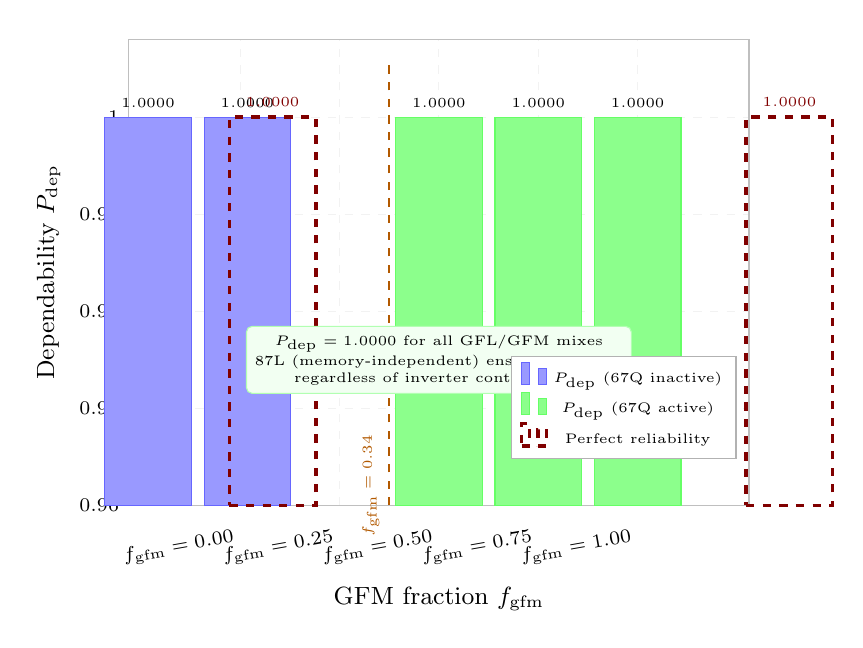
\begin{tikzpicture}
\begin{axis}[
  name         = covax,
  width        = 0.78\textwidth,
  height       = 7.5cm,
  ybar,
  bar width    = 1.1cm,
  xlabel       = {GFM fraction $f_\mathrm{gfm}$},
  ylabel       = {Dependability $P_\mathrm{dep}$},
  xlabel style = {font=\small},
  ylabel style = {font=\small},
  ymin=0.96, ymax=1.008,
  ytick        = {0.96,0.97,0.98,0.99,1.00},
  yticklabel style={font=\scriptsize},
  xtick        = {1,2,3,4,5},
  xticklabels  = {$f_\mathrm{gfm}=0.00$,
                  $f_\mathrm{gfm}=0.25$,
                  $f_\mathrm{gfm}=0.50$,
                  $f_\mathrm{gfm}=0.75$,
                  $f_\mathrm{gfm}=1.00$},
  xticklabel style={font=\scriptsize, rotate=10, anchor=north east},
  tick style   = {draw=none},
  axis line style={gray!50},
  grid         = major,
  grid style   = {gray!10, dashed},
  nodes near coords,
  nodes near coords style={font=\tiny, anchor=south},
  every node near coord/.append style={
    /pgf/number format/.cd, fixed, fixed zerofill, precision=4
  },
  legend style={at={(0.98,0.10)}, anchor=south east, font=\tiny,
                draw=gray!60, fill=white},
  clip=false,
]

%% P_dep bars — all 1.0000, but vary colour by 67Q-active status
%  f_gfm=0.00,0.25: 67Q inactive (f < 0.34); blue
%  f_gfm=0.50,0.75,1.00: 67Q active; green

\addplot[fill=blue!40, draw=blue!60]
  coordinates {(1,1.0000) (2,1.0000)};
\addlegendentry{$P_\mathrm{dep}$ (67Q inactive)}

\addplot[fill=green!45, draw=green!60]
  coordinates {(3,1.0000) (4,1.0000) (5,1.0000)};
\addlegendentry{$P_\mathrm{dep}$ (67Q active)}

%% Perfect reference line
\addplot[red!50!black, dashed, very thick, mark=none]
  coordinates {(0.4, 1.0) (5.6, 1.0)};
\addlegendentry{Perfect reliability}

%% 67Q activation boundary
\draw[orange!70!black, thick, dashed]
  (axis cs:2.5, 0.960) -- (axis cs:2.5, 1.006);
\node[orange!70!black, font=\tiny, rotate=90, anchor=south]
  at (axis cs:2.5, 0.962)
  {$f_\mathrm{gfm}=0.34$};

%% Annotation
\node[draw=green!30, fill=green!5, rounded corners=2pt,
      font=\tiny, inner sep=3pt, align=center]
  at (axis cs:3, 0.975)
  {$P_\mathrm{dep}=1.0000$ for all GFL/GFM mixes\\
   87L (memory-independent) ensures coverage\\
   regardless of inverter control mode};

\end{axis}
\end{tikzpicture}
